\documentclass{article}
\usepackage[utf8]{inputenc}
\usepackage{geometry}
\usepackage{longtable}
\usepackage{graphicx} % For including images
\usepackage{hyperref} % For hyperlinks
\usepackage{enumitem}
\usepackage{graphicx}
\usepackage{booktabs} % For professional looking tables
\usepackage{float} % For improved control over floating environments

\geometry{
 a4paper,
 total={170mm,257mm},
 left=20mm,
 top=20mm,
}

\title{Laboratory Assignment 1: Deployment View of Mathpix}
\author{Can Acay}
\date{\today}

\begin{document}

\maketitle
\newpage

\tableofcontents
\newpage

\section{Software System Selection}
Mathpix is an OCR (Optical Character Recognition) service designed to extract textual information from images. Its purpose is to accurately convert images of typed or handwritten math problems into editable text and render LaTeX code for mathematical expressions. Key functionalities include image preprocessing, text recognition, LaTeX rendering, and handling user interactions through various client applications.

\section{Quality Attributes and System Requirements}
The Mathpix system should be designed to meet the following key quality attributes and system requirements:

\subsection{Performance}
\begin{itemize}
\item The OCR service should process images and generate LaTeX code within an acceptable response time, typically under 2 seconds for average-sized images.
\item The system should be able to handle a high volume of concurrent requests without significant performance degradation.
\item Caching mechanisms should be implemented to improve response times for frequently accessed results.
\end{itemize}

\subsection{Scalability}
\begin{itemize}
\item The system should be designed to scale horizontally, allowing the addition of more instances to handle increased traffic and processing demands.
\item The microservices architecture should enable independent scaling of individual components based on their specific resource requirements.
\item The system should be able to accommodate a growing user base and increasing usage without compromising performance or availability.
\end{itemize}

\subsection{Reliability}
\begin{itemize}
\item The system should have high availability, with a minimum uptime of 99.9% to ensure uninterrupted service to users.
\item Fault tolerance mechanisms should be implemented to handle component failures gracefully, without impacting the overall system functionality.
\item Regular backups and disaster recovery procedures should be in place to minimize data loss and enable quick recovery in case of failures.
\end{itemize}

\subsection{Security}
\begin{itemize}
\item User authentication and authorization should be enforced to protect user data and prevent unauthorized access.
\item Secure communication protocols (HTTPS) should be used for all data transmissions between components and client applications.
\item Sensitive user information and processed data should be encrypted at rest and in transit to maintain confidentiality.
\item Regular security audits and vulnerability assessments should be conducted to identify and mitigate potential security risks.
\end{itemize}

\section{Component Identification}
Mathpix is built with a range of components that work together to provide a robust service:

\begin{itemize}
    \item \textbf{Client Applications}: Interfaces include a web application, a mobile app, and a desktop program, each designed to meet different user needs.
    \item \textbf{Input Handlers}: Tools to handle various types of inputs, including keyboard for text, images for scanning, handwriting recognition, and PDF text extraction.
    \item \textbf{Authenticator Service}: Ensures users can securely access their accounts.
    \item \textbf{API Gateway}: Serves as the hub for all client requests, efficiently managing traffic and optimizing system response.
    \item \textbf{Rate Limiter and Response Cache}: Helps maintain system stability by controlling the flow of requests and caching data to speed up responses.
    \item \textbf{Monitoring \& Analytics Server}: Keeps an eye on system health and gathers data to help improve the service.
    \item \textbf{Databases}: Stores various types of data, including user information, input records, performance metrics, and cached LaTeX renderings.
    \item \textbf{OCR Service}: Recognizes text in images and converts it into an editable format.
    \item \textbf{LaTeX Rendering}: Takes the text from the OCR and turns it into LaTeX format, ready for use in academic and scientific documents.
\end{itemize}


\section{Deployment Models and Nodes}
\begin{enumerate}
    \item \textbf{Client Application (Public Cloud or User Devices):}
    The client applications, such as web, mobile, or desktop apps, should be deployed on public cloud platforms or run directly on user devices. This allows easy access for users to interact with the Mathpix service.
    
    \item \textbf{API Gateway (Public Cloud):}
    The API Gateway should be deployed on a public cloud to handle incoming requests from client applications. It acts as the entry point for the system, routing requests to the appropriate services.

    \item \textbf{Load Balancer (Public Cloud):}
    The load balancer should be deployed on a public cloud to distribute incoming traffic across multiple instances of the API Gateway, OCR Service, and LaTeX Rendering components.
    
    \item \textbf{Authenticator Service (Private Cloud or Dedicated Server):}
    The Authenticator Service should be deployed on a private cloud or dedicated server to ensure the security of user authentication and authorization processes. Keeping it separate from public-facing components adds an extra layer of security.
    
    \item \textbf{OCR Service (Private Cloud or Dedicated Server):}
    The OCR Service, which performs the core functionality of image processing and text recognition, should be deployed on a private cloud or dedicated server. This ensures better control over the processing resources and allows for scalability and performance optimization.
    
    \item \textbf{Input Database (Private Cloud or Dedicated Server):}
    The Input Database, which stores the processed images and extracted text, should be deployed on a private cloud or dedicated server. This keeps the data secure and allows for efficient access by the OCR Service.
    
    \item \textbf{Monitoring \& Analytics Server (Private Cloud or Dedicated Server):}
    The Monitoring \& Analytics Server should be deployed on a private cloud or dedicated server to collect and process system metrics and logs. This allows for centralized monitoring and analysis of the system's performance and usage.
    
    \item \textbf{Metrics \& Logs Database (Private Cloud or Dedicated Server):}
    The Metrics \& Logs Database should be deployed on a private cloud or dedicated server to store the collected metrics and logs. This ensures data security and allows for efficient querying and analysis.
    
    \item \textbf{Analytics Database (Private Cloud or Dedicated Server):}
    The Analytics Database, which stores user behavior and system usage data, should be deployed on a private cloud or dedicated server. This keeps the data secure and allows for efficient access by the Analytics Server.
    
    \item \textbf{LaTeX Rendering (Private Cloud or Dedicated Server):}
    The LaTeX Rendering component should be deployed on a private cloud or dedicated server to handle the rendering of mathematical expressions into LaTeX code. This ensures better control over the rendering process and allows for scalability.
    
    \item \textbf{User Database (Private Cloud or Dedicated Server):}
    The User Database, which stores user account information, should be deployed on a private cloud or dedicated server to ensure the security and privacy of user data.
    
    \item \textbf{Image Processing (Private Cloud or Dedicated Server):}
    The Image Processing component, which performs tasks like noise reduction, binarization, and normalization, should be deployed on a private cloud or dedicated server. This allows for efficient processing and scalability of the image preprocessing tasks.
\end{enumerate}

\section{Deployment Patterns and Styles Analysis}
Based on the identified components and the chosen deployment models and nodes, the following deployment patterns and styles can be applied to the Mathpix system:

\subsection{Client-Server Pattern}
The Mathpix system can follow a client-server pattern, where the client applications (web, mobile, and desktop) interact with the server-side components through the API Gateway. The client applications send requests to the server, which processes them and returns the appropriate responses. This pattern allows for a clear separation of concerns between the client and server, enabling scalability and maintainability.

\subsection{Microservices Architecture}
The Mathpix system can be designed using a microservices architecture, where the system is decomposed into smaller, loosely coupled services. Each component, such as the OCR Service, LaTeX Rendering, Image Processing, and various databases, can be developed and deployed as independent microservices. This architecture promotes modularity, flexibility, and scalability, as each microservice can be scaled and updated independently based on the specific requirements.

\subsection{API Gateway Pattern}
The API Gateway acts as the entry point for all client requests and serves as a single interface to the underlying microservices. It handles request routing, composition, and protocol translation. The API Gateway can also implement cross-cutting concerns such as authentication, rate limiting, and caching. This pattern simplifies client communication and provides a unified API for the Mathpix system.

\subsection{Database per Service Pattern}
Each microservice in the Mathpix system can have its own dedicated database, following the Database per Service pattern. This allows each service to have its own data model and schema, optimized for its specific requirements. The User Database, Input Database, Metrics \& Logs Database, and Analytics Database can be deployed separately and accessed by their respective services, ensuring data isolation and scalability.

\subsection{Event-Driven Architecture}
The Mathpix system can incorporate an event-driven architecture to enable asynchronous communication between microservices. Events can be used to trigger actions and data flow between services. For example, when an image is processed by the OCR Service, it can publish an event containing the extracted text. The LaTeX Rendering service can subscribe to this event and render the LaTeX code asynchronously. This pattern promotes loose coupling and enables scalability and fault tolerance.

\section{Deployment Tactics Evaluation}
To achieve specific quality attributes in the Mathpix system, the following deployment tactics can be evaluated:

\subsection{Horizontal Scaling}
Horizontal scaling can be applied to improve the performance and scalability of the Mathpix system. The API Gateway, OCR Service, and LaTeX Rendering components can be deployed across multiple instances, with a load balancer distributing the incoming requests among them. This allows the system to handle increased traffic and ensures high availability. Kubernetes or other container orchestration platforms can be used to manage the deployment and scaling of these components.

\subsection{Caching}
Caching can be implemented at various levels to improve the performance and reduce the load on the backend services. The API Gateway can include a response cache to store frequently accessed results, such as rendered LaTeX code or recognized text. This reduces the need to process the same requests repeatedly. Additionally, the LaTeX Rendering service can maintain a cache of rendered expressions to serve them quickly for subsequent requests. Caching can significantly improve response times and reduce the overall system load.

\subsection{Monitoring and Logging}
Comprehensive monitoring and logging should be implemented to ensure the reliability and observability of the Mathpix system. The Monitoring \& Analytics Server can collect metrics and logs from various components and store them in the Metrics \& Logs Database. This allows for real-time monitoring of system health, performance, and usage. Tools like Prometheus and Grafana can be used for collecting and visualizing metrics, while the ELK stack (Elasticsearch, Logstash, Kibana) can be employed for centralized logging and analysis. Alerts can be set up based on predefined thresholds to proactively identify and resolve issues.

\begin{figure}[H]
    \centering
    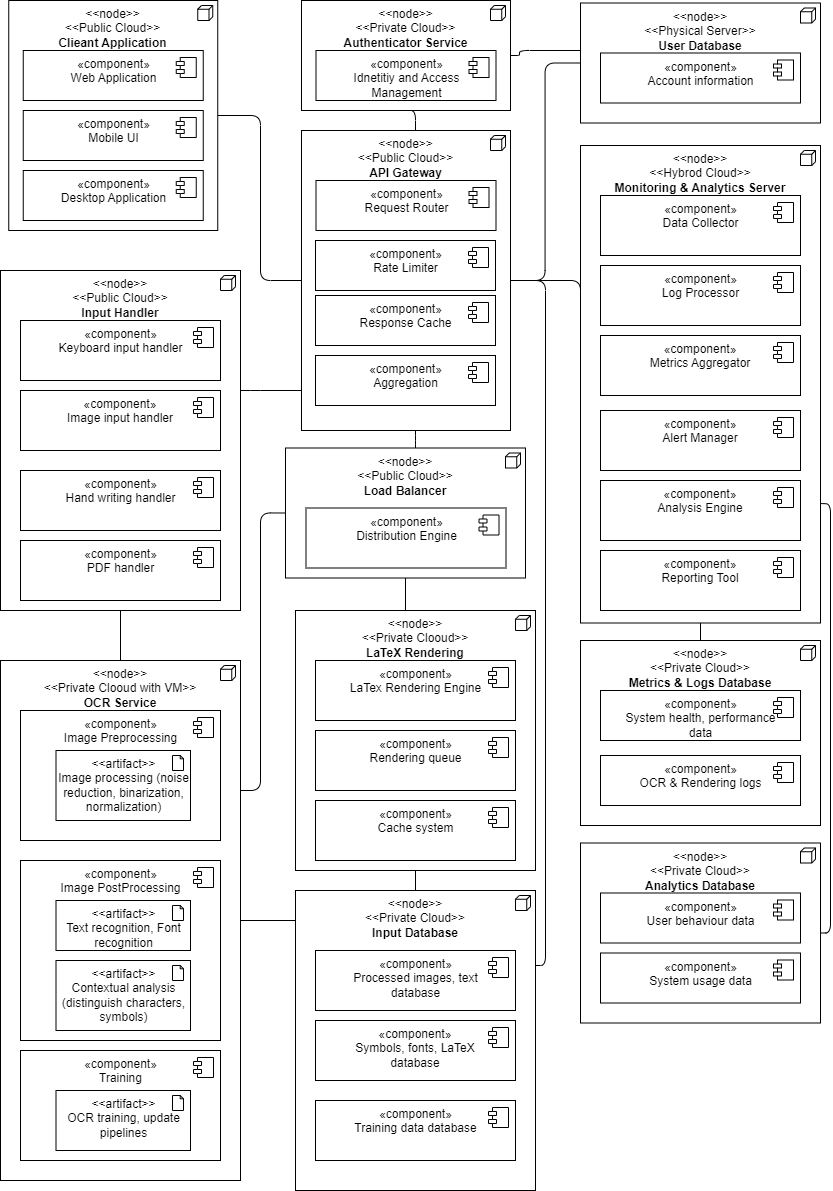
\includegraphics[width=\textwidth]{deployment_diagram.png}
    \caption{Deployment Diagram of Mathpix}
    \label{fig:Deployment Diagram of Mathpix}
\end{figure}

\section{Report}
\subsection{Analysis Summary}
The deployment of the Mathpix system has been carefully designed to ensure high performance, scalability, reliability, and security. The system follows a microservices architecture pattern, which allows for the decomposition of the system into smaller, loosely coupled services. This approach promotes modularity, flexibility, and maintainability, as each microservice can be developed, deployed, and scaled independently based on its specific requirements.

The client applications, such as the web, mobile, and desktop apps, interact with the system through the API Gateway, which serves as the single entry point for all client requests. The API Gateway acts as a reverse proxy, routing requests to the appropriate microservices based on the request path or parameters. It also handles cross-cutting concerns such as authentication, rate limiting, and caching, simplifying client communication and providing a unified API for the Mathpix system.

To ensure high availability and scalability, the API Gateway, OCR Service, and LaTeX Rendering components are deployed across multiple instances using a load balancer. The load balancer distributes incoming traffic evenly among the instances, allowing the system to handle increased loads and ensuring optimal performance. Horizontal scaling is employed to dynamically adjust the number of instances based on the demand, enabling the system to accommodate a growing user base and increasing usage without compromising performance or availability.

The deployment diagram showcases a clear separation between the public-facing components (client applications and API Gateway) and the internal microservices and databases. The public-facing components are deployed on a public cloud infrastructure, providing easy access for users and enabling seamless interaction with the Mathpix service. On the other hand, the core microservices and databases, such as the OCR Service, LaTeX Rendering, Image Processing, and various databases, are deployed on a private cloud or dedicated servers. This deployment approach enhances security and control over sensitive data and critical processing tasks.

To further improve performance and reduce the load on backend services, caching mechanisms are implemented at various levels. The API Gateway includes a response cache to store frequently accessed results, such as rendered LaTeX code or recognized text. This eliminates the need to process the same requests repeatedly, significantly reducing response times. Additionally, the LaTeX Rendering service maintains a cache of rendered expressions, allowing for quick retrieval of previously rendered content.


To ensure the reliability and observability of the Mathpix system, comprehensive monitoring and logging mechanisms are implemented. The Monitoring \& Analytics Server collects metrics and logs from various components and stores them in the Metrics \& Logs Database. This enables real-time monitoring of system health, performance, and usage. Tools like Prometheus and Grafana are employed for collecting and visualizing metrics, while the ELK stack (Elasticsearch, Logstash, Kibana) is used for centralized logging and analysis. Alerts are set up based on predefined thresholds to proactively identify and resolve any issues, minimizing downtime and ensuring a smooth user experience.

\subsection{Rationale for Deployment Patterns, Styles, and Tactics}
The deployment patterns, styles, and tactics chosen for the Mathpix system are based on a careful consideration of the system requirements and desired quality attributes.

The microservices architecture pattern is selected to achieve modularity, scalability, and maintainability. By breaking down the system into smaller, loosely coupled services, each component can be developed, deployed, and scaled independently. This allows for faster development cycles, easier updates, and the ability to scale individual components based on their specific resource requirements.

The client-server pattern is employed to establish a clear separation between the client applications and the server-side components. This separation allows for better security, as the server-side components can be deployed on a private cloud or dedicated servers, protecting sensitive data and critical processing tasks.

The API Gateway pattern is chosen to provide a single entry point for all client requests and to handle cross-cutting concerns. It simplifies client communication, enables request routing, and allows for the implementation of common functionalities such as authentication, rate limiting, and caching.

The database per service pattern is selected to ensure data isolation and allow each microservice to have its own optimized data model and schema. This approach prevents data coupling between services and enables independent scaling and evolution of each service's data storage.

Horizontal scaling and load balancing are employed to achieve high performance and availability. By distributing the load across multiple instances of the API Gateway, OCR Service, and LaTeX Rendering components, the system can handle increased traffic and ensure optimal response times. Horizontal scaling allows for dynamic adjustment of resources based on demand, ensuring the system can accommodate a growing user base and increasing usage.

Caching is implemented to improve performance and reduce the load on backend services. By caching frequently accessed results, such as rendered LaTeX code or recognized text, the system can serve requests faster and minimize unnecessary processing.

Monitoring and logging are crucial for ensuring the reliability and observability of the system. By collecting metrics and logs from various components and storing them in a centralized database, the system can be proactively monitored for any issues or anomalies. Real-time monitoring and alerting enable quick identification and resolution of problems, minimizing downtime and ensuring a smooth user experience.

\subsection{Alignment with System Requirements and Quality Attributes}
The deployment choices made for the Mathpix system align well with the identified system requirements and desired quality attributes.

Performance is achieved through horizontal scaling, load balancing, and caching. By distributing the load across multiple instances and caching frequently accessed results, the system can handle a high volume of concurrent requests and deliver fast response times.

Scalability is addressed through the microservices architecture and horizontal scaling. The system can easily scale individual components based on their specific resource requirements, allowing it to accommodate a growing user base and increasing usage without compromising performance or availability.

Reliability is ensured through the separation of concerns between public-facing and internal components, as well as comprehensive monitoring and logging. By deploying critical services on a private cloud or dedicated servers and implementing real-time monitoring and alerting, the system can proactively identify and resolve issues, minimizing downtime and ensuring a reliable user experience.

Security is enhanced by deploying the Authenticator Service on a separate, secure server and using secure communication protocols and data encryption. The separation of public-facing and internal components further protects sensitive data and critical processing tasks.

In conclusion, the deployment patterns, styles, and tactics chosen for the Mathpix system align well with the system requirements and desired quality attributes. The microservices architecture, client-server pattern, API Gateway, database per service pattern, horizontal scaling, caching, monitoring, and logging all contribute to achieving high performance, scalability, reliability, and security. By carefully designing the deployment architecture and selecting appropriate patterns and tactics, the Mathpix system is well-positioned to deliver a robust and efficient OCR service to its users.

\end{document}
